\documentclass[12pt]{article}
\input{doc/header/header}
\input{doc/header/defs}

\usepackage[utf8]{inputenc} % allow utf-8 input
\usepackage[T1]{fontenc}    % use 8-bit T1 fonts
\usepackage{url}            % simple URL typesetting
\usepackage{booktabs}       % professional-quality tables
\usepackage{amsfonts}       % blackboard math symbols
\usepackage{nicefrac}       % compact symbols for 1/2, etc.
\usepackage{microtype}      % microtypography
\usepackage{lipsum}
\graphicspath{ {./images/} }
\usepackage[margin=2.5cm,nohead]{geometry}
\usepackage{authblk}
\newcommand{\email}[1]{\href{mailto:#1}{#1}}
\usepackage[final]{pdfpages}

\title{\RtEstim: Time-varying reproduction number estimation with trend filtering}

\author[a,1]{Jiaping Liu}
\author[b]{Zhenglun Cai}
\author[a]{Paul Gustafson}
\author[a]{Daniel J. McDonald}

\affil[a]{Department of Statistics, The University of British Columbia}
\affil[b]{Centre for Health Evaluation and Outcome Sciences, The University of
British Columbia}

\begin{document}

\maketitle

\begin{abstract}
  To understand the transmissibility and spread of infectious diseases,
epidemiologists turn to estimates of the instantaneous reproduction number.
While many estimation approaches exist, their utility may be limited. 
Challenges of surveillance data collection, model assumptions
that are unverifiable with data alone, and 
computationally inefficient frameworks are critical limitations for many
existing approaches. We propose a discrete spline-based approach that solves a convex optimization problem---Poisson trend filtering---using the proximal Newton method. It produces a locally adaptive 
estimator for instantaneous reproduction number estimation with heterogeneous 
smoothness. Our methodology remains accurate even under some process 
misspecifications and is computationally efficient, even for large-scale 
data. The implementation is easily accessible in a lightweight \R\ 
package \href{https://dajmcdon.github.io/rtestim/index.html}{\texttt{rtestim}}.

  {\bf Keywords:} Reproduction number $|$ infectious disease $|$ discrete spline $|$ trend filtering
\end{abstract}


\footnotetext[1]{To whom correspondence should be
  addressed. E-mail: \email{jiaping.liu@stat.ubc.ca}} 


\clearpage

\input{doc/introduction}  
\input{doc/methods}
\input{doc/results}
\input{doc/discussion}



\section*{Acknowledgments}

This research was enabled in part by support provided by 
BC DRI group who manages Cedar cloud (https://docs.alliancecan.ca/wiki/Cedar)
and the Digital Research Alliance of Canada (alliancecan.ca).



\addcontentsline{toc}{section}{References}

\bibliographystyle{doc/rss.bst}
\bibliography{doc/rt}


%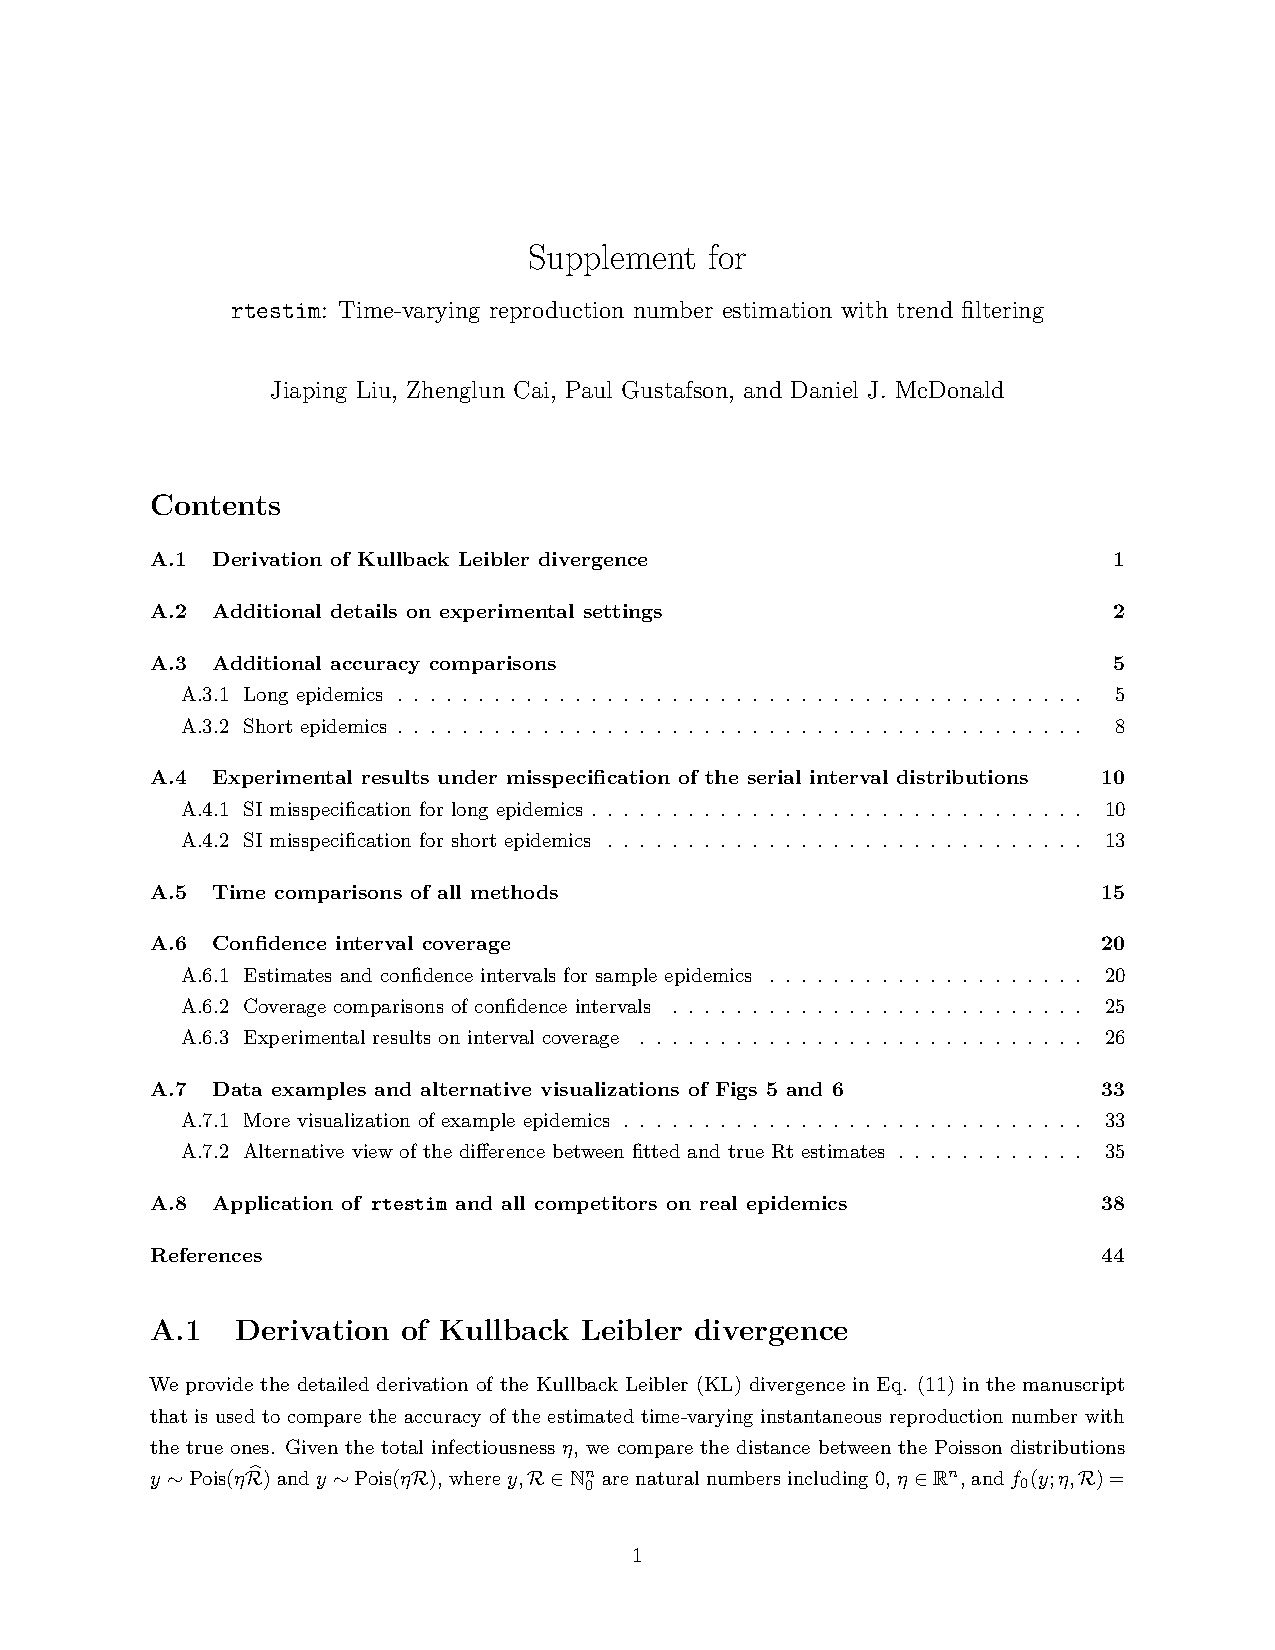
\includepdf[pages=-]{src/supp.pdf}

\end{document}
